\qrchapter{https://forgottenpillar.com/rsc/en-fp-chapter8}{The constructive criticism}


\qrchapter{https://forgottenpillar.com/rsc/en-fp-chapter8}{النقد البناء}


The first point of the \emcap{Fundamental Principles} answers the questions: who is God, what is His personality, and how do we understand His presence?


تجيب النقطة الأولى من \emcap{المبادئ الأساسية} على الأسئلة: من هو الله، وما هي شخصانيته، وكيف نفهم حضوره؟


\others{I. That there is \textbf{one God}, \textbf{a personal, spiritual }\textbf{\underline{being}}, \textbf{the creator of all things}, omnipotent, omniscient, and eternal; infinite in wisdom, holiness, justice, goodness, truth, and mercy; unchangeable, and \textbf{everywhere present by his representative, the Holy Spirit}. Ps. 139:7.}[FP1889 147.2; 1889][https://egwwritings.org/read?panels=p931.6]


\others{I. أن هناك \textbf{إله واحد}، \textbf{كائن شخصي روحي}\textbf{\underline{}}، \textbf{خالق كل الأشياء}، كلي القدرة، كلي العلم، وأبدي؛ غير محدود في الحكمة، والقداسة، والعدل، والصلاح، والحق، والرحمة؛ لا يتغير، و\textbf{حاضر في كل مكان بواسطة ممثله، الروح القدس}. مز 139: 7.}[FP1889 147.2; 1889][https://egwwritings.org/read?panels=p931.6]


The one God, the Creator, is identified as the Father, because the second point of the \emcap{Fundamental Principles} states that Jesus Christ, the Son of the Eternal Father, is the one by whom God created all things\footnote{\href{https://egwwritings.org/?ref=en_FP1889.147.3&para=931.7}{FP1889 147.3; 1889}}. The \emcap{personality of God} is expressed in the term “\textit{personal spiritual being}”. We will soon see that this term denotes that the Father has a material body, a physical manifestation. Thus, in His personality, He is present only where He dwells physically. But, His presence is not constrained to His personality because He is \others{everywhere present by his representative, the Holy Spirit}. During our past history, this understanding and reasoning of the \emcap{personality of God}, as expressed in the first point of the \emcap{Fundamental Principles}, received constructive criticism; by “constructive criticism” we refer to the criticism supported by the Bible.


الإله الواحد، الخالق، يُعرَّف بأنه الآب، لأن النقطة الثانية من \emcap{المبادئ الأساسية} تنص على أن يسوع المسيح، ابن الآب الأبدي، هو الذي به خلق الله كل الأشياء\footnote{\href{https://egwwritings.org/?ref=en_FP1889.147.3&para=931.7}{FP1889 147.3; 1889}}. يتم التعبير عن \emcap{شخصانية الله} في مصطلح “\textit{كائن شخصي روحي}”. سنرى قريبًا أن هذا المصطلح يشير إلى أن الآب له جسد مادي، مظهر فيزيائي. وبالتالي، في شخصانيته، هو موجود فقط حيث يسكن جسديًا. لكن حضوره لا يقتصر على شخصانيته لأنه \others{حاضر في كل مكان بواسطة ممثله، الروح القدس}. خلال تاريخنا الماضي، تلقى هذا الفهم والتفكير في \emcap{شخصانية الله}، كما هو معبر عنه في النقطة الأولى من \emcap{المبادئ الأساسية}، نقدًا بناءً؛ بـ “النقد البناء” نشير إلى النقد المدعوم بالكتاب المقدس.


We now present to you the following citations, some constructive criticism, from a prominent trinitarian brother in the Seventh-day Adventist world. Interestingly, he had acknowledged the authority of the \emcap{Fundamental Principles}, yet simultaneously believed in the Trinity doctrine. We find this document a very important element in the change of our beliefs from the fundamental principles to current Seventh-day Adventist Trinitarian belief.


نقدم لكم الآن الاقتباسات التالية، بعض النقد البناء، من أخ ثالوثي بارز في عالم الأدفنتست السبتيين. من المثير للاهتمام أنه اعترف بسلطة \emcap{المبادئ الأساسية}، ومع ذلك آمن في الوقت نفسه بعقيدة الثالوث. نجد هذه الوثيقة عنصرًا مهمًا جدًا في تغيير معتقداتنا من المبادئ الأساسية إلى معتقد الأدفنتست السبتيين الثالوثي الحالي.


This prominent brother was met with the question, “\textit{Do you not believe in a personal, definite God?}”:


واجه هذا الأخ البارز السؤال، “\textit{ألا تؤمن بإله شخصي ومحدد؟}”:


\others{\textbf{Most certainly. An infinite, divine, personal being is essential religion}. Worship requires someone to love, to obey, to trust. \textbf{Belief in a personal God is the very core of the Christian religion}. The conception of God as the All-Energy, the infinite Power, an all-pervading Presence, is too vast for the human mind to grasp; there must be something more \textbf{tangible}, more \textbf{\underline{restricted}}, upon which to center the mind in worship. \textbf{It is for this reason that Christ came to us in the image of God's }\textbf{\underline{personality}}\textbf{, the second Adam, to show us by his life of love and self-sacrifice the character and }\textbf{\underline{the personality of God}}. We can approach God only through Christ.}


\others{\textbf{بالتأكيد. كائن شخصي إلهي غير محدود هو أساس الدين}. العبادة تتطلب شخصًا ما لنحبه، ونطيعه، ونثق به. \textbf{الإيمان بإله شخصي هو جوهر الديانة المسيحية}. مفهوم الله باعتباره الطاقة الكلية، القوة اللامتناهية، حضور منتشر في كل مكان، هو أمر أكبر من أن يستوعبه العقل البشري؛ يجب أن يكون هناك شيء أكثر \textbf{ملموسية}، أكثر \textbf{\underline{تحديدًا}}، لتركيز العقل عليه في العبادة. \textbf{لهذا السبب جاء المسيح إلينا على صورة }\textbf{\underline{شخصانية}}\textbf{ الله، آدم الثاني، ليظهر لنا من خلال حياته المليئة بالمحبة والتضحية بالنفس صفة و}\textbf{\underline{شخصانية الله}}. يمكننا الاقتراب من الله فقط من خلال المسيح.}


\othersnogap{‘Who being the brightness of his glory, and \textbf{the express image of his person}, and upholding all things by the word of his power, when he had by himself purged our sins, sat down on the right hand of the Majesty on high.’}


\othersnogap{‘الذي، وهو بهاء مجده، و\textbf{صورة جوهره}، وحامل كل الأشياء بكلمة قدرته، بعدما صنع بنفسه تطهيرًا لخطايانا، جلس في يمين العظمة في الأعالي.’}


\othersnogap{‘Who being the effulgence of his glory, and the impress of his substance, and upholding all things by the word of his power.’}


\othersnogap{‘الذي هو إشعاع مجده، وطبعة جوهره، وحامل كل الأشياء بكلمة قدرته.’}


\othersnogap{The apostle says, ‘But we all, with open face \textbf{beholding as in a glass} the glory of the Lord, are changed into the same image from glory to glory, even as by the Spirit of the Lord.’ 2 Cor. 3: 18. How apt and beautiful is this figure!... So, \textbf{in beholding Christ} in his miracles, his temptations, his exhortations, his life of self-abnegation, his ‘going about doing good,’ \textbf{we may behold the personality and power of God}. And what a great hope there is for us in the fact that \textbf{in Christ we find qualities not strange and foreign to humanity}, but kindred mental and moral characteristics; so that we are able to see and grasp an actual, rather than merely a theological or abstract or figurative truth, in the declaration of the apostle, ‘Now are we the sons of God.’ 1 John 3:2.}


\othersnogap{يقول الرسول: ‘ونحن جميعًا \textbf{ناظرين كما في مرآة} مجد الرب، نتغير إلى تلك الصورة عينها، من مجد إلى مجد، كما من الرب الروح.’ 2 كور 3: 18. ما أدق وأجمل هذا التشبيه!... هكذا، \textbf{بالنظر إلى المسيح} في معجزاته، وتجاربه، ومواعظه، وحياته في إنكار الذات، و'تجوله يصنع خيرًا’، \textbf{يمكننا أن نرى شخصانية وقوة الله}. وما أعظم الرجاء لنا في حقيقة أننا \textbf{نجد في المسيح صفات ليست غريبة وأجنبية عن البشرية}، بل خصائص عقلية وأخلاقية مماثلة؛ حتى نتمكن من رؤية وفهم حقيقة فعلية، وليست مجرد حقيقة لاهوتية أو مجردة أو مجازية، في إعلان الرسول، ‘الآن نحن أولاد الله.’ 1 يوحنا 3: 2.}


\othersnogap{\textbf{The fact that God is so great that we cannot form a clear mental picture of his }\textbf{\underline{physical appearance}}\textbf{ need not lessen in our minds the reality of }\textbf{\underline{His personality}}\textbf{, neither does this conception disagree with that of a special expression of God in some }\textbf{\underline{particular form or place}}. \textbf{\underline{Indeed, there are scriptures which present God in this definite, and one may say circumscribed, form as sitting upon a throne in heaven, or as dwelling in the temple at Jerusalem}}, 1. Kings 22:19; Ps. 11:4; Matt. 21:12, 13.}


\othersnogap{\textbf{إن حقيقة أن الله عظيم لدرجة أننا لا نستطيع تكوين صورة ذهنية واضحة عن }\textbf{\underline{مظهره الجسدي}}\textbf{ لا ينبغي أن تقلل في أذهاننا من واقع }\textbf{\underline{شخصانيته}}\textbf{، ولا يتعارض هذا المفهوم مع ذلك التعبير الخاص عن الله في }\textbf{\underline{شكل أو مكان معين}}. \textbf{\underline{في الواقع، هناك نصوص كتابية تقدم الله في هذا الشكل المحدد، وقد يقول المرء المحدود، كجالس على عرش في السماء، أو كساكن في الهيكل في أورشليم}}، 1 ملوك 22:19؛ مزمور 11:4؛ متى 21:12، 13.}


\othersnogap{The human mind is finite and cannot grasp infinity. \textbf{We naturally desire to form a definite, clearly defined conception of the being whom we worship}. \textbf{The Bible supplies this human need as well as all other of our spiritual requirements, and }\textbf{\underline{in the fortieth chapter of Isaiah}}\textbf{ the prophet deals with this question of God's personal appearance in a marvelous way}. ‘O Jerusalem, that bringest good tiding, lift up thy voice with strength; lift it up, be not afraid; say unto the cities of Judah, \textbf{Behold your God}! He shall feed his flock like a shepherd: he shall gather the lambs in his arms, and carry them in his bosom.’}


\othersnogap{العقل البشري محدود ولا يستطيع إدراك اللانهاية. \textbf{نحن بطبيعتنا نرغب في تكوين مفهوم محدد وواضح المعالم عن الكائن الذي نعبده}. \textbf{يلبي الكتاب المقدس هذه الحاجة البشرية وكذلك جميع متطلباتنا الروحية الأخرى، و}\textbf{\underline{في الفصل الأربعين من إشعياء}}\textbf{ يتناول النبي مسألة المظهر الشخصي لله بطريقة رائعة}. ‘يا أورشليم، التي تبشرين بأخبار سارة، ارفعي صوتك بقوة؛ ارفعيه، لا تخافي؛ قولي لمدن يهوذا، \textbf{هوذا إلهكم}! سيرعى قطيعه كراعٍ: سيجمع الحملان في ذراعيه، ويحملهم في حضنه.’}


\othersnogap{‘Who hath measured the waters in the hollow of \textbf{his hand}, and meted out heaven with the span, and comprehended the dust of the earth in a measure, and weighed the mountains in scales, and the hills in a balance? \textbf{To whom then will ye liken God?} \textbf{Or what likeness will ye compare unto him?} Have ye not known? have ye not heard? hath it not been told you from the beginning? have ye not understood from the foundations of the earth? \textbf{It is he that sitteth upon the circle of the earth}, and the inhabitants thereof are as grasshoppers; \textbf{that stretcheth out the heavens as a curtain, and spreadeth them out as a tent to dwell in}: \textbf{\underline{To whom then will ye liken me, or shall I be equal? saith the Holy One}}. Lift up your eyes on high, and behold who hath created these things, that bringeth out their host by number: he calleth them all by names by the greatness of his might, for that he is strong in power; not one faileth. Hast thou not known? hast thou not heard, that the everlasting God, the Lord, the Creator of the ends of the earth, fainteth not, neither is weary? There is no searching of his understanding. He giveth power to the faint and to them that have no might he increaseth strength. Even the youths shall faint and be weary, and the young men shall utterly fall: but they that wait upon the Lord shall renew their strength; they shall mount up with wings as eagles; they shall run, and not be weary; and they shall walk, and not faint.’ Isa. 40:9,11,12,18,21,22,25,26,28-31.}


\othersnogap{‘من كال المياه بكف \textbf{يده}، وقاس السماوات بالشبر، وكال تراب الأرض بالكيل، ووزن الجبال بالقبان، والتلال بالميزان؟ \textbf{فبمن تشبهون الله؟} \textbf{وأي شبه تعادلون به؟} ألم تعلموا؟ ألم تسمعوا؟ ألم تخبروا من البداية؟ ألم تفهموا من أساسات الأرض؟ \textbf{هو الجالس على دائرة الأرض}، وسكانها كالجراد؛ \textbf{الذي ينشر السماوات كسرادق، ويبسطها كخيمة للسكن}: \textbf{\underline{فبمن تشبهونني فأساويه؟ يقول القدوس}}. ارفعوا عيونكم إلى العلاء وانظروا من خلق هذه، الذي يخرج جندها بعدد: يدعوها كلها بأسماء لعظمة قوته، لكونه شديد القوة؛ لا يفقد أحد. ألم تعلم؟ ألم تسمع، أن الإله الأبدي، الرب، خالق أطراف الأرض، لا يكل ولا يعيا؟ ليس عن فهمه فحص. يعطي المعيي قدرة ولعديم القوة يكثر شدة. الغلمان يعيون ويتعبون، والفتيان يتعثرون تعثرًا: أما منتظرو الرب فيجددون قوتهم؛ يرتفعون بأجنحة كالنسور؛ يركضون ولا يتعبون؛ يمشون ولا يعيون.’ إشعياء 40:9،11،12،18،21،22،25،26،28-31.}


\othersnogap{\textbf{Here is a most marvelous description of God. His hand, his arm, his bosom are mentioned}. He is described as ‘sitting on the circle of the earth,’ he metes out heaven with the span, he holds the waters in the hollow of his hand; \textbf{\underline{so there can be no question that God is a definite, real, personal being}}. \textbf{A mere abstract principle, a law, a force could not have a hand, an arm. \underline{God is a person}, though too great for us to comprehend, as Job says}, ‘God is great and we know him not.’ Job 36:26...}


\othersnogap{\textbf{هنا وصف رائع جدًا لله. يُذكر يده، ذراعه، حضنه}. يوصف بأنه ‘جالس على دائرة الأرض’، يقيس السماء بالشبر، يمسك المياه في كف يده؛ \textbf{\underline{لذلك لا يمكن أن يكون هناك أي شك في أن الله كائن حقيقي، محدد، شخصي}}. \textbf{مجرد مبدأ مجرد، قانون، قوة لا يمكن أن يكون لها يد، ذراع. \underline{الله شخص}، رغم أنه عظيم جدًا بحيث لا يمكننا فهمه، كما يقول أيوب}، ‘هوذا الله عظيم ولا نعرفه.’ أيوب 36:26...}


\othersnogap{\textbf{\underline{This great being} is represented as sitting on the circle of the earth}. The orbit of the earth is nearly two hundred million miles in diameter. \textbf{A being so great as to occupy a seat of such proportions is quite \underline{beyond our comprehension as regards his form}}. \textbf{The prophet recognizes this, and so \underline{diverts our attention away from speculation respecting the exact size and form of God} by showing us the absurdity of trying to form even a mental image, \underline{intimating that this is closely akin to idolatry}. See verses 18-21}. He then shows us where to find a true conception of God, pointing us to the things which he has made: ‘Lift up your eyes on high and behold who hath created these things.’ This also was Paul's idea : ‘For the invisible things of him from the creation of the world are clearly seen, being understood by the things that are made, \textbf{even his eternal power and \underline{Godhead}}; so that they are without excuse.’ Rom. 1:20.}


\othersnogap{\textbf{\underline{هذا الكائن العظيم} يُصوَّر جالسًا على دائرة الأرض}. يبلغ قطر مدار الأرض ما يقرب من مائتي مليون ميل. \textbf{كائن عظيم لدرجة أنه يشغل مقعدًا بهذه الأبعاد هو \underline{أبعد من فهمنا فيما يتعلق بشكله}}. \textbf{يدرك النبي هذا، ولذلك \underline{يحول انتباهنا بعيدًا عن التكهنات المتعلقة بالحجم والشكل الدقيقين لله} من خلال إظهار عبثية محاولة تكوين صورة ذهنية، \underline{مشيرًا إلى أن هذا قريب جدًا من عبادة الأصنام}. انظر الآيات 18-21}. ثم يوضح لنا أين نجد مفهومًا حقيقيًا عن الله، مشيرًا إلينا الأشياء التي صنعها: ‘ارفعوا أعينكم إلى العلاء وانظروا من خلق هذه’. كانت هذه أيضًا فكرة بولس: ‘لأن أموره غير المنظورة تُرى منذ خلق العالم مدركة بالمصنوعات، \textbf{قدرته السرمدية و\underline{لاهوته}}؛ حتى إنهم بلا عذر.’ رومية 1:20.}


\othersnogap{\textbf{\underline{Discussions respecting the form of God are utterly unprofitable}, and serve only to belittle our conceptions of him who is above all things}, \textbf{and hence not to be compared in form or size or glory or majesty with anything which man has ever seen or which it is within his power to conceive}. In the presence of questions like these, we have only to acknowledge our foolishness and incapacity, and bow our heads with awe and reverence \textbf{in the presence of a Personality, an Intelligent Being} to the existence of which all nature bears definite and positive testimony, \textbf{but which is as far beyond our comprehension \underline{as are the bounds of space and time}}.}


\othersnogap{\textbf{\underline{المناقشات المتعلقة بشكل الله عديمة الفائدة تمامًا}، ولا تخدم سوى تصغير مفاهيمنا عنه الذي هو فوق كل الأشياء}، \textbf{وبالتالي لا يمكن مقارنته في الشكل أو الحجم أو المجد أو العظمة بأي شيء رآه الإنسان أو في قدرته أن يتصوره}. في حضرة أسئلة كهذه، ليس لدينا سوى الاعتراف بحماقتنا وعجزنا، وخفض رؤوسنا بخشية وتوقير \textbf{في حضرة شخصانية، كائن ذكي} تشهد له كل الطبيعة شهادة محددة وإيجابية، \textbf{لكنه بعيد عن فهمنا \underline{كما هي حدود الزمان والمكان}}.}


As mentioned before, this brother acknowledges the \emcap{Fundamental Principles}, yet believes in the Trinity. Here is a short summary of His constructive criticism regarding the \emcap{personality of God}: God is a definite, real, personal being, having a form—\others{\textbf{Indeed, there are scriptures which present God in \underline{this definite}, and one may say \underline{circumscribed}, form as sitting upon a throne in heaven}}. He advocates this because he believes it is necessary for us, finite human beings, to have a definite object of worship. But he expands the idea of a “\textit{circumscribed} God by the testimony from Isaiah chapter 40, which proves that God is\others{\textbf{\underline{beyond our comprehension as regards his form}}}. Any kind of conceptualization of God’s being, in any form, is akin to idolatry. \others{\textbf{\underline{Discussions respecting the form of God are utterly unprofitable}}}. The true matter of the personality of infinite God is beyond our comprehension. God’s true personality is more than a mystery to our finite minds. This is because God is\others{\textbf{far beyond our comprehension \underline{as are the bounds of space and time}}}. For this brother, understanding God’s personality merely as a definite being is in one way true, but in another way false. It is true that God presented Himself in \others{\textbf{\underline{particular form or place}}}, because \others{there must be something more \textbf{tangible}, more \textbf{\underline{restricted}}, upon which to center the mind in worship}. A simple understanding of God as a definite and tangible being is restrictive for God. The summary of his criticism is that we should form our conceptions of God outside of \others{\textbf{the bounds of space and time}}.


كما ذكرنا سابقًا، هذا الأخ يقر بـ\emcap{المبادئ الأساسية}، ومع ذلك يؤمن بالثالوث. فيما يلي ملخص موجز لانتقاده البناء فيما يتعلق بـ\emcap{شخصانية الله}: الله كائن محدد، حقيقي، شخصي، له شكل—\others{\textbf{في الواقع، هناك نصوص كتابية تقدم الله في \underline{هذا الشكل المحدد}، وقد يقول المرء \underline{المحدود}، كجالس على عرش في السماء}}. يدافع عن هذا لأنه يعتقد أنه من الضروري لنا، نحن البشر المحدودين، أن يكون لدينا هدف محدد للعبادة. لكنه يوسع فكرة الله “\textit{المحدود} من خلال الشهادة من إشعياء الفصل 40، الذي يثبت أن الله \others{\textbf{\underline{أبعد من فهمنا فيما يتعلق بشكله}}}. أي نوع من تصور كيان الله، بأي شكل، يشبه عبادة الأصنام. \others{\textbf{\underline{المناقشات المتعلقة بشكل الله عديمة الفائدة تمامًا}}}. المسألة الحقيقية لشخصانية الله اللانهائي تتجاوز فهمنا. شخصانية الله الحقيقية هي أكثر من لغز لعقولنا المحدودة. هذا لأن الله \others{\textbf{بعيد عن فهمنا \underline{كما هي حدود الزمان والمكان}}}. بالنسبة لهذا الأخ، فإن فهم شخصانية الله كمجرد كائن محدد صحيح من ناحية، وخاطئ من ناحية أخرى. صحيح أن الله قدم نفسه في \others{\textbf{\underline{شكل أو مكان معين}}}, لأنه \others{يجب أن يكون هناك شيء أكثر \textbf{ملموسية}، أكثر \textbf{\underline{تقييدًا}}، لتركيز العقل عليه في العبادة}. الفهم البسيط لله ككائن محدد وملموس هو تقييد لله. ملخص انتقاده هو أننا يجب أن نشكل مفاهيمنا عن الله خارج \others{\textbf{حدود الزمان والمكان}}.


Please, candidly examine the reasons behind this brother’s faith. The reasoning behind his arguments is important to understand because it played an important role in Seventh-day Adventist history, as a bold step away from the \emcap{Fundamental Principles}. These arguments are not trivial; they are very persuasive and we urge you to their contemplation. Perhaps you might agree with them, but please allow us to unmask the deception. These citations are from Dr. Kellogg’s book “\textit{The Living Temple}”\footnote{\href{https://archive.org/details/J.H.Kellogg.TheLivingTemple1903}{Dr. J. H. Kellogg, The Living Temple, p.29-33.}}. From the section titled “\textit{Infinite Intelligence a Personal being}”, pages 29 to 33, the passages express Kellogg’s position on the \emcap{personality of God}, which was the main problem with his book.


من فضلك، افحص بصدق الأسباب وراء إيمان هذا الأخ. المنطق وراء حججه مهم للفهم لأنه لعب دورًا مهمًا في تاريخ كنيسة الأدفنتست السبتيين، كخطوة جريئة بعيدًا عن \emcap{المبادئ الأساسية}. هذه الحجج ليست تافهة؛ إنها مقنعة جدًا وندعوك إلى التفكير فيها. ربما توافق عليها، لكن يرجى السماح لنا بكشف الخداع. هذه الاقتباسات من كتاب الدكتور كيلوغ “\textit{ذا ليفينغ تمبل}”\footnote{\href{https://archive.org/details/J.H.Kellogg.TheLivingTemple1903}{Dr. J. H. Kellogg, The Living Temple, p.29-33.}}. من القسم المعنون “\textit{الذكاء اللانهائي كائن شخصي}”، الصفحات من 29 إلى 33، تعبر المقاطع عن موقف كيلوغ بشأن \emcap{شخصانية الله}، وهي المشكلة الرئيسية في كتابه.


That which you just read was exactly what Sister White referred to when she said: \egwinline{I have some things to say to our teachers \textbf{in reference to the new book The Living Temple}. \textbf{Be careful how you sustain the sentiments of this book \underline{regarding the personality of God}}. As the Lord presents matters to me, \textbf{these sentiments do not bear the endorsement of God}. \textbf{They are a snare that the enemy has prepared for these last days}...}[Lt211-1903.1; 1903][https://egwwritings.org/read?panels=p9598.8]


ما قرأته للتو هو بالضبط ما أشارت إليه الأخت وايت عندما قالت: \egwinline{لدي بعض الأشياء لأقولها لمعلمينا \textbf{فيما يتعلق بالكتاب الجديد ذا ليفينغ تمبل}. \textbf{كونوا حذرين في كيفية دعمكم للآراء الواردة في هذا الكتاب \underline{بخصوص شخصانية الله}}. كما يقدم الرب الأمور لي، \textbf{فإن هذه الآراء لا تحمل تأييد الله}. \textbf{إنها فخ أعده العدو لهذه الأيام الأخيرة}...}[Lt211-1903.1; 1903][https://egwwritings.org/read?panels=p9598.8]


In the present Seventh-day Adventist controversy over the Trinity doctrine, we have personally been trying to shift the controversy from the Trinity doctrine to the \emcap{personality of God}. We’ve presented the position of the first point of the \emcap{Fundamental Principles} and have encountered arguments that greatly overlap with Dr. Kellogg’s sentiment on the \emcap{personality of God}, advocated in “\textit{Living Temple}”. We’ve seen this repeatedly. When the focus is drawn from the Trinity issue to the \emcap{personality of God}, Kellogg’s views regarding the \emcap{personality of God} frequently echoe from the lips of Trinitarian advocates. The quality or state of God being a person is a mystery in the Trinity doctrine, and often Kellogg’s sentiment on the \emcap{personality of God} resonates with Trinitarian understanding of God’s person.


في الجدل الحالي في كنيسة الأدفنتست السبتيين حول عقيدة الثالوث، كنا نحاول شخصيًا تحويل الجدل من عقيدة الثالوث إلى \emcap{شخصانية الله}. لقد قدمنا موقف النقطة الأولى من \emcap{المبادئ الأساسية} وواجهنا حججًا تتداخل بشكل كبير مع رأي الدكتور كيلوغ حول \emcap{شخصانية الله}، الذي دافع عنه في “\textit{ذا ليفينغ تمبل}”. لقد رأينا هذا مرارًا وتكرارًا. عندما يتم تحويل التركيز من قضية الثالوث إلى \emcap{شخصانية الله}، غالبًا ما تتردد آراء كيلوغ بشأن \emcap{شخصانية الله} من شفاه المدافعين عن الثالوث. الصفة أو الحالة التي يكون بها الله شخصًا هي لغز في عقيدة الثالوث، وغالبًا ما يتردد صدى رأي كيلوغ حول \emcap{شخصانية الله} مع الفهم الثالوثي لشخص الله.


\begin{figure}[hp]
    \centering
    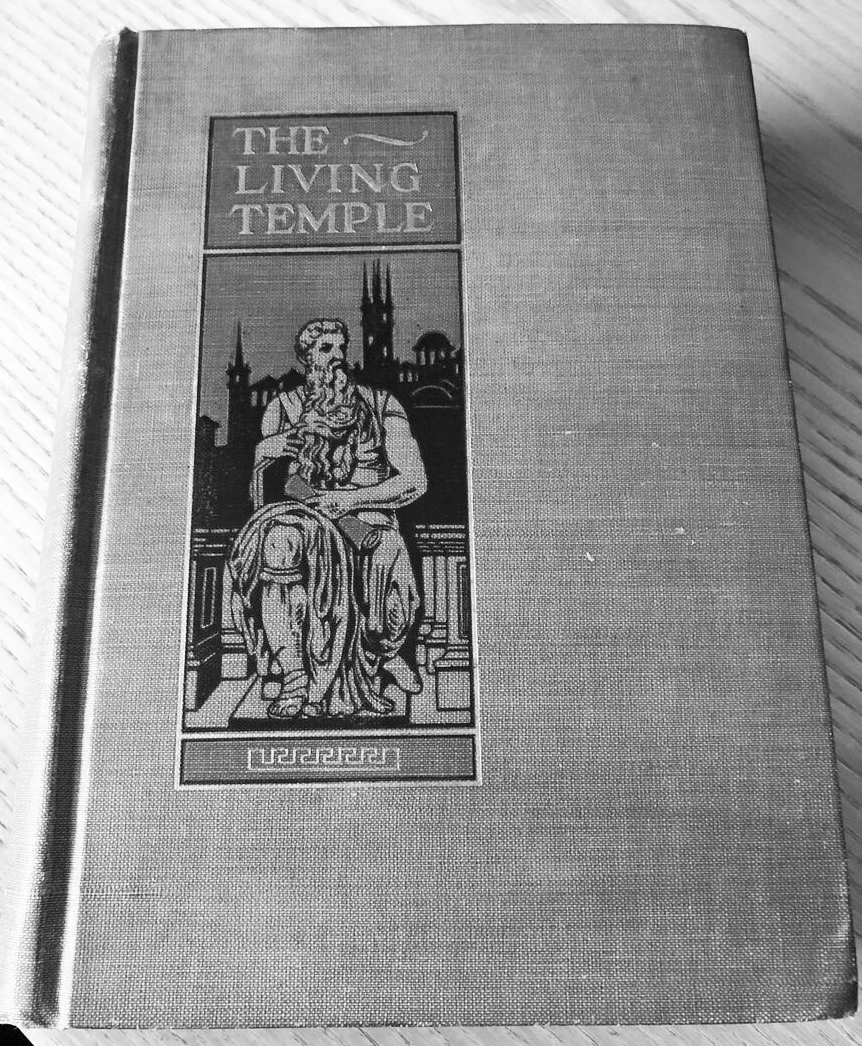
\includegraphics[width=1\linewidth]{images/TLT.jpg}
    \caption*{The Living Temple by Dr. J. H. Kellogg, 1903}
    \label{fig:tlt}
\end{figure}


\begin{figure}[hp]
    \centering
    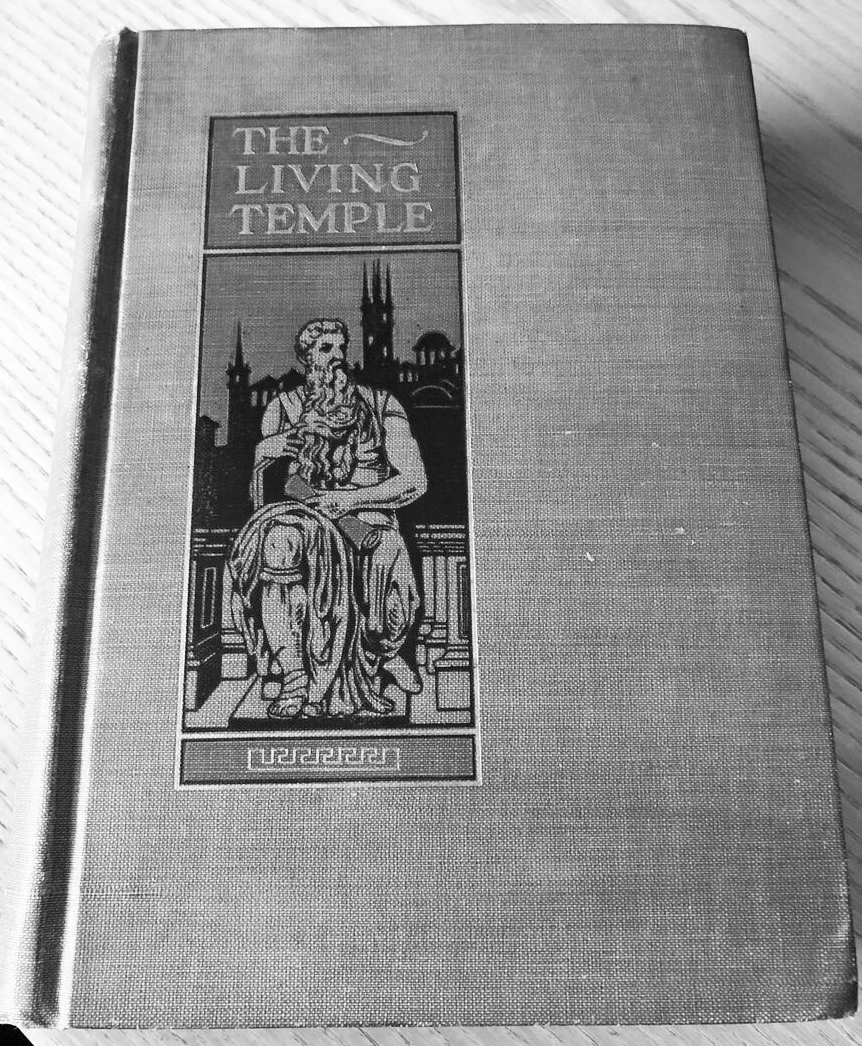
\includegraphics[width=1\linewidth]{images/TLT.jpg}
    \caption*{ذا ليفينغ تمبل للدكتور ج. هـ. كيلوغ، 1903}
    \label{fig:tlt}
\end{figure}


Some people find Dr. Kellogg’s understanding of God’s personality resonates with their understanding, yet they are tempted to think that there are other things objectionable with the Living Temple. The following evidence suggests the very opposite. There is a letter from Dr. Kellogg to William C. White, where Dr. Kellogg proposes to \others{cutting out a few leaves} from the three thousand copies of the Living Temple—those very leaves containing the \others{specially objectionable things appear, such as the comment on Isaiah 40} and the sentiments regarding the \emcap{personality of God} (the pages we have read).


يجد بعض الناس أن فهم الدكتور كيلوغ لشخصانية الله يتوافق مع فهمهم، ومع ذلك فهم معرضون للتفكير بأن هناك أشياء أخرى مرفوضة في كتاب ذا ليفينغ تمبل. الأدلة التالية تشير إلى العكس تمامًا. هناك رسالة من الدكتور كيلوغ إلى ويليام سي. وايت، حيث يقترح الدكتور كيلوغ \others{قص بعض الصفحات} من ثلاثة آلاف نسخة من كتاب ذا ليفينغ تمبل—تلك الصفحات التي تحتوي على \others{الأشياء المرفوضة بشكل خاص، مثل التعليق على إشعياء 40} والآراء المتعلقة بـ\emcap{شخصانية الله} (الصفحات التي قرأناها).


\others{The Sanitarium has on hand, I find, \textbf{two or three thousand books which were sold}, but which have come back since the book was condemned. The question has been raised, what shall be done with these? \textbf{It has occurred to me that perhaps they might be saved \underline{by cutting out a few leaves} in which the \underline{specially objectionable things appear}, such as the \underline{comment on Isaiah 40}, which I borrowed from A.T. Jones, and the page on which the unfortunate heading appears, ‘\underline{The Personality of God},’ and tipping in leaves embodying a clear statement of the Bible view of God as a person presented in Elder Haskell’s article in the ‘Review’ a few weeks ago}. These books would be sold to old patients who are making a great demand for the book for Christmas presents…}[Letter from Dr. J.H. Kellogg to W.C.White; December 6, 1903, Chicago][https://174625.selcdn.ru/ellenwhite/EWhite/17226/17226.pdf]


\others{المصح لديه، كما وجدت، \textbf{ألفين أو ثلاثة آلاف كتاب تم بيعها}، لكنها عادت منذ أن تم إدانة الكتاب. السؤال الذي طُرح هو: ماذا سنفعل بهذه الكتب؟ \textbf{خطر لي أنه ربما يمكن إنقاذها \underline{بقص بعض الصفحات} التي تظهر فيها \underline{الأشياء المرفوضة بشكل خاص}، مثل \underline{التعليق على إشعياء 40}، الذي استعرته من إيه.تي. جونز، والصفحة التي يظهر فيها العنوان المؤسف، ‘\underline{شخصانية الله}،‘ وإلصاق صفحات تتضمن بيانًا واضحًا لوجهة نظر الكتاب المقدس عن الله كشخص كما قدمها الشيخ هاسكل في مقاله في ‘ريفيو’ قبل بضعة أسابيع}. سيتم بيع هذه الكتب للمرضى القدامى الذين يطلبون الكتاب بشدة كهدايا عيد الميلاد...}[رسالة من الدكتور ج.هـ. كيلوغ إلى دبليو.سي.وايت؛ 6 ديسمبر 1903، شيكاغو][https://174625.selcdn.ru/ellenwhite/EWhite/17226/17226.pdf]


What is the real issue with the reasoning in the Living Temple? We will study the matter to its very depth; superficially, we clearly see that the issue is the stepping off of the foundation of our faith—the \emcap{Fundamental Principles}—regarding the \emcap{personality of God} and where His presence is.


ما هي المشكلة الحقيقية في المنطق الوارد في كتاب ذا ليفينغ تمبل؟ سندرس المسألة إلى أعمق مستوياتها؛ سطحيًا، نرى بوضوح أن المشكلة هي الخروج عن أساس إيماننا—\emcap{المبادئ الجوهرية}—فيما يتعلق بـ\emcap{شخصانية الله} وأين يوجد حضوره.


\egw{\textbf{I have been instructed by the heavenly messenger} that \textbf{some of the reasoning} in the book, ‘Living Temple’, is unsound and that \textbf{this reasoning would lead astray} the minds of those who are not thoroughly established on \textbf{the foundation principles} of present truth. \textbf{It introduces that which is naught but speculation} in \textbf{regard to the personality of God and where His presence is}.}[SpTB02 51.3; 1904][https://egwwritings.org/read?panels=p417.262]


\egw{\textbf{لقد تلقيت تعليمات من الرسول السماوي} أن \textbf{بعض المنطق} في كتاب ‘ذا ليفينغ تمبل’ غير سليم وأن \textbf{هذا المنطق سيضلل} عقول أولئك الذين ليسوا راسخين تمامًا على \textbf{المبادئ الأساسية} للحق الحاضر. \textbf{إنه يقدم ما هو مجرد تكهنات} فيما \textbf{يتعلق بشخصانية الله وأين يوجد حضوره}.}[SpTB02 51.3; 1904][https://egwwritings.org/read?panels=p417.262]


Dr. Kellogg introduced the thought \egwinline{which is naught but speculation in regard to the personality of God}, by which he stepped off of the foundation of our faith—the \emcap{Fundamental Principles}. Discordance between Dr. Kellogg’s teaching and the \emcap{Fundamental Principles} is in the first statement of the principles where we are taught that\others{That there is \textbf{one God}, \textbf{a personal, spiritual \underline{being}}, \textbf{the creator of all things}, ... and \textbf{everywhere present by his representative, the Holy Spirit}. Ps. 139:7.}


قدم الدكتور كيلوغ الفكرة \egwinline{التي هي مجرد تكهنات فيما يتعلق بشخصانية الله}، والتي بها خرج عن أساس إيماننا—\emcap{المبادئ الجوهرية}. التناقض بين تعاليم الدكتور كيلوغ و\emcap{المبادئ الجوهرية} يكمن في البيان الأول من المبادئ حيث نُعلَّم أن \others{هناك \textbf{إله واحد}، \textbf{كائن شخصي روحي}، \textbf{خالق كل الأشياء}، ... و\textbf{موجود في كل مكان بواسطة ممثله، الروح القدس}. مزمور 139: 7.}


Sister White directly warned us of the sentiments expressed in the Living Temple regarding the \emcap{personality of God}. They are not in harmony with the first point of the \emcap{Fundamental Principles}, which were part of the foundation of our faith.


حذرتنا الأخت وايت مباشرة من الآراء المعبر عنها في كتاب ذا ليفينغ تمبل فيما يتعلق بـ\emcap{شخصانية الله}. هذه الآراء ليست متوافقة مع النقطة الأولى من \emcap{المبادئ الجوهرية}، التي كانت جزءًا من أساس إيماننا.


\egw{\textbf{I have had to write much concerning the strange doctrines and theories expressed in Living Temple. \underline{Were these theories accepted by our people, the strong pillars of our faith and the truths that have made Seventh-day Adventists what they are would be swept away}. I have had to show the fallacy of these doctrines, presenting them \underline{as a species of last-day heresy}. We are told by the Word of God that just such teaching \underline{will be brought in at this time}.}}[Lt250-1903.2; 1903][https://egwwritings.org/read?panels=p9337.8]


\egw{\textbf{كان عليّ أن أكتب الكثير بخصوص العقائد والنظريات الغريبة المعبر عنها في كتاب ذا ليفينغ تمبل. \underline{لو قبل شعبنا هذه النظريات، لتم اكتساح الأعمدة القوية لإيماننا والحقائق التي جعلت الأدفنتست السبتيين ما هم عليه}. كان عليّ أن أبين خطأ هذه العقائد، مقدمة إياها \underline{كنوع من الهرطقة في الأيام الأخيرة}. يخبرنا كلام الله أن مثل هذا التعليم بالضبط \underline{سيتم تقديمه في هذا الوقت}.}}[Lt250-1903.2; 1903][https://egwwritings.org/read?panels=p9337.8]


Today we witness the widespread acceptance of Kellogg’s theories regarding the \emcap{personality of God}. The fact that the first point of the \emcap{Fundamental Principles} is no longer present in our beliefs proves that Kellogg’s theories regarding the \emcap{personality of God} have had an influence in shaping our beliefs.


نشهد اليوم قبولًا واسع النطاق لنظريات كيلوغ المتعلقة بـ\emcap{شخصانية الله}. حقيقة أن النقطة الأولى من \emcap{المبادئ الجوهرية} لم تعد موجودة في معتقداتنا تثبت أن نظريات كيلوغ المتعلقة بـ\emcap{شخصانية الله} كان لها تأثير في تشكيل معتقداتنا.


\egw{One and another come to me, asking me to \textbf{explain the positions taken in “Living Temple.”} I reply, “They are unexplainable.” \textbf{The sentiments expressed do not give a true knowledge of God.} \textbf{All through the book are passages of scripture}. \textbf{These scriptures are brought in in such a way \underline{that error is made to appear as truth}}. \textbf{Erroneous theories are presented in so pleasing a way that unless care is taken, many will be misled}.}[SpTB02 52.1; 1904][https://egwwritings.org/read?panels=p417.265]


\egw{يأتي إليّ واحد تلو الآخر، يطلبون مني \textbf{شرح المواقف المتخذة في “ذا ليفينغ تمبل.”} أجيب، “إنها غير قابلة للشرح.” \textbf{الآراء المعبر عنها لا تعطي معرفة حقيقية بالله.} \textbf{في جميع أنحاء الكتاب توجد مقاطع من الكتاب المقدس}. \textbf{هذه النصوص الكتابية تم إدراجها بطريقة \underline{تجعل الخطأ يبدو كأنه حقيقة}}. \textbf{يتم تقديم النظريات الخاطئة بطريقة جذابة لدرجة أنه ما لم يتم توخي الحذر، سيضل الكثيرون}.}[SpTB02 52.1; 1904][https://egwwritings.org/read?panels=p417.265]


The error is being made to appear as truth, and many are misled.


يظهر الخطأ وكأنه الحقيقة، ويضل كثيرون.


It is worth emphasizing, for some careless reader, that the real issue of Dr. Kellogg, and his book “\textit{Living Temple}”, is not the Trinity but the small step he took off of the \emcap{Fundamental Principles}. In order to understand the real issue of his book, it would be wrong to focus on its overlapping sentiments with the Trinity doctrine. Rather, we should focus on the point that constituted this small step he made; and this includes having a deep understanding of the \emcap{fundamental principles} just as our pioneers had. Who better to ask than the Adventist pioneers themselves?


من الجدير بالتأكيد، لبعض القراء غير المنتبهين، أن القضية الحقيقية للدكتور كيلوغ وكتابه “\textit{Living Temple}”، ليست الثالوث بل الخطوة الصغيرة التي اتخذها بعيدًا عن \emcap{المبادئ الجوهرية}. ولفهم القضية الحقيقية لكتابه، سيكون من الخطأ التركيز على آرائه المتداخلة مع عقيدة الثالوث. بل يجب أن نركز على النقطة التي شكلت هذه الخطوة الصغيرة التي اتخذها؛ وهذا يتضمن فهمًا عميقًا \emcap{للمبادئ الجوهرية} كما فهمها روادنا. ومن أفضل من نسأله من الرواد الأدفنتست أنفسهم؟


% Constructive Criticism

\begin{titledpoem}
    
    \stanza{
        A personal God in heaven sits enthroned, \\
        This truth in our Principles firmly zoned. \\
        Present everywhere by Spirit's might, \\
        This foundation stood as our guiding light.
    }

    \stanza{
        Then came words that seemed so wise and deep, \\
        A subtle shift that made the faithful weep. \\
        "God's form beyond all human thought," they claimed, \\
        A mystery too vast to be contained or named.
    }

    \stanza{
        "Discussions of God's form," the Temple said, \\
        "Are futile paths where idols lie ahead." \\
        Yet this philosophy so smoothly spun, \\
        Was the very snare by which souls were won.
    }

    \stanza{
        The error dressed as truth appeared so fair, \\
        As scripture twisted in a clever snare. \\
        One small step from the Principles we held, \\
        One giant leap by which our faith was felled.
    }

    \stanza{
        Beware the mind that thinks itself too wise, \\
        To see deception veiled in truth's disguise. \\
        God is personal, definite, and real, \\
        This is the truth the Temple would conceal. 
    }
\end{titledpoem}